\section{Ionic mit Cordova beziehungsweise Capacitor}
\label{sec:Frameworks_Ionic}

Das Ionic-Framework ist selbst kein Cross-Plattform Framework, sondern ein UI-Toolkit  \cite{Ionic_Docs}.
Damit unterstützt Ionic die Cross-Plattform Entwicklung nur indirekt, indem insbesondere die Erstellung der Oberflächen vereinfacht wird.
Wie \autoref{fig:ionic_architecture} zeigt, ist Ionic auf ein unterlagertes Cross-Plattform Framework angewiesen.
Hierfür unterstützt Ionic Apache Cordova und das vom Ionic-Team entwickelte Capacitor, wobei die Verwendung des moderneren Capacitor empfohlen wird.
Da Capacitor von Ionic als Weiterentwicklung von Cordova angesehen wird, wird in \autoref{sec:Cordova_Capacitor} auch kurz auf Capacitor eingegangen, obwohl es nicht als eines der populärsten Frameworks gilt.
Ionic lässt sich allerdings auch in reinen Webanwendungen nutzen \cite{Ionic_Docs}.
\begin{figure}[h]
    \centering
    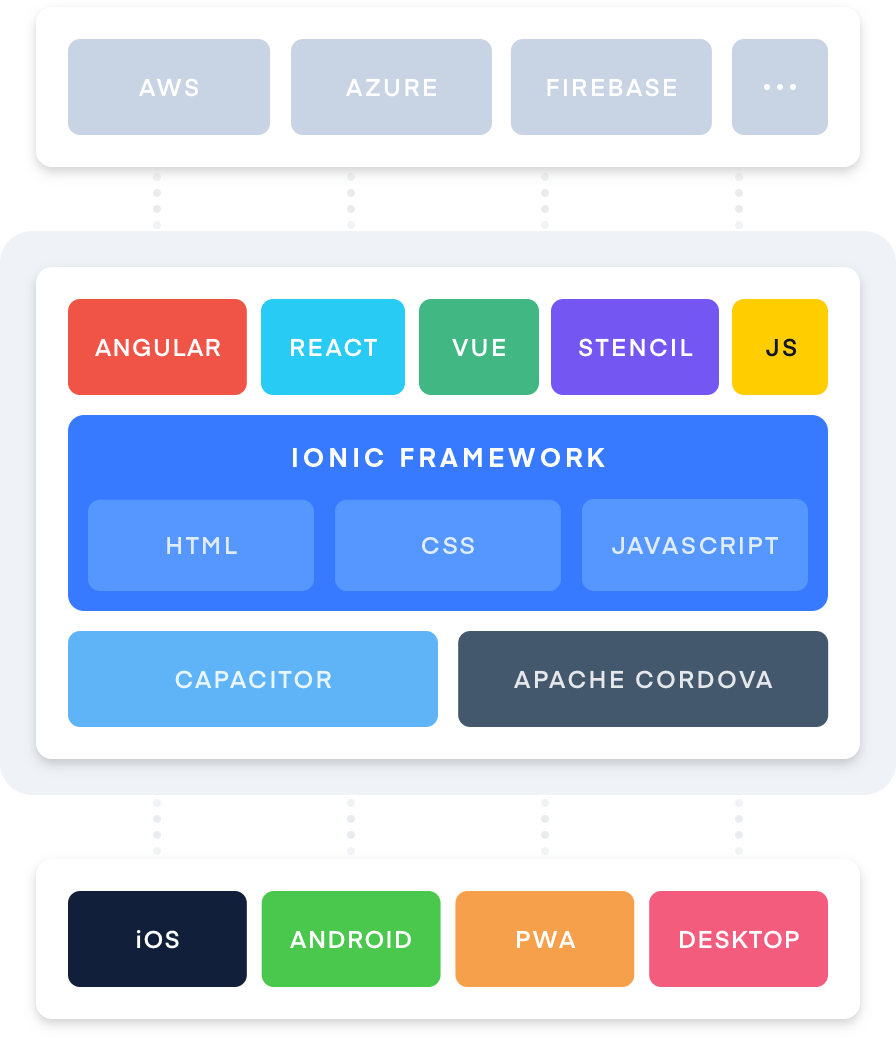
\includegraphics[clip, trim=0cm 0cm 0 8cm,height=8cm]{ionic_architecture.png}
    \caption{Architektur des Ionic-Frameworks \cite{Ionic_Architektur}}
    \label{fig:ionic_architecture}
\end{figure}
Ionic stellt \ac{UI}-Komponenten zur Verfügung, die plattformübergreifend genutzt werden können und automatisch dem Stil der jeweiligen Plattform angepasst werden.
Zur weiteren Vereinfachung bietet Ionic die Unterstützung der beliebten Frontend-Frameworks und Bibliotheken Angular, React und Vue.js.
Eine Ionic-Anwendung lässt sich allerdings auch mit anderen Frontend-Technologien oder komplett ohne Frontend-Framework erstellen \cite{Ionic_Docs, Ionic_EvaluationGuide}.
Ein weiterer Vorteil der Verwendung von Cordova oder Capacitor in Verbindung mit Ionic sind die angebotenen Zusatzleistungen.
Für zahlende Kunden bietet Ionic persönliche Beratung und Support, ein eigenes \ac{CD} System und proprietäre Plugins für verschiedene Funktionen, die nicht über Open-Source Plugins abgedeckt werden können \cite{Ionic_EvaluationGuide}.


\subsection{Apache Cordova und Capacitor}
\label{sec:Cordova_Capacitor}
Die beiden unterstützen Cross-Plattform Frameworks Cordova und Capacitor sind sich im Allgemeinen sehr ähnlich.
Beide ermöglichen es, Webanwendungen in native Anwendungen einzubetten und über ein Plugin-System auf native \acp{API} zuzugreifen \cite{Ionic_Cordova_vs_Capacitor}.


Apache Cordova ist das deutlich ältere Framework und wird als Open-Source-Projekt von der Apache Software Foundation verwaltet.
Eine Open-Source Version des ursprünglich kommerziellen Frameworks \textit{PhoneGap} wurde 2011 an die Apache Software Foundation übergeben \cite{Steyer_Cordova}.
Die kommerzielle Version des Frameworks wurde bis 2020 vertrieben, die Open-Source Variante wird weiter entwickelt \cite{Adobe_PhoneGap_EOL}.


Zur Unterstützung mehrerer Plattformen verwendet Cordova den Ansatz einer Hybrid Web App.
Jede Web-App, welche mit \ac{HTML}, \ac{CSS} und JavaScript entwickelt wurde, lässt sich mit Cordova als native Anwendung verpacken.
Theoretisch sind Web-Apps auch ohne den Einsatz von Cordova bereits plattformunabhängig, da sie auf verschiedenen Plattformen im Browser ausgeführt werden können.
Mit Cordova kann auf den Umweg über den Browser verzichtet werden und die Anwendung lässt sich über den App-Store der jeweiligen Plattform verbreiten.
Dazu verwendet Cordova eine Wrapper-Anwendung, welche die eigentliche Web-App in einer WebView ausführt.
\autoref{fig:cordova_architecture} zeigt die Architektur, die sich durch diese Einbettung der Web-App ergibt.
\begin{figure}[h]
    \centering
    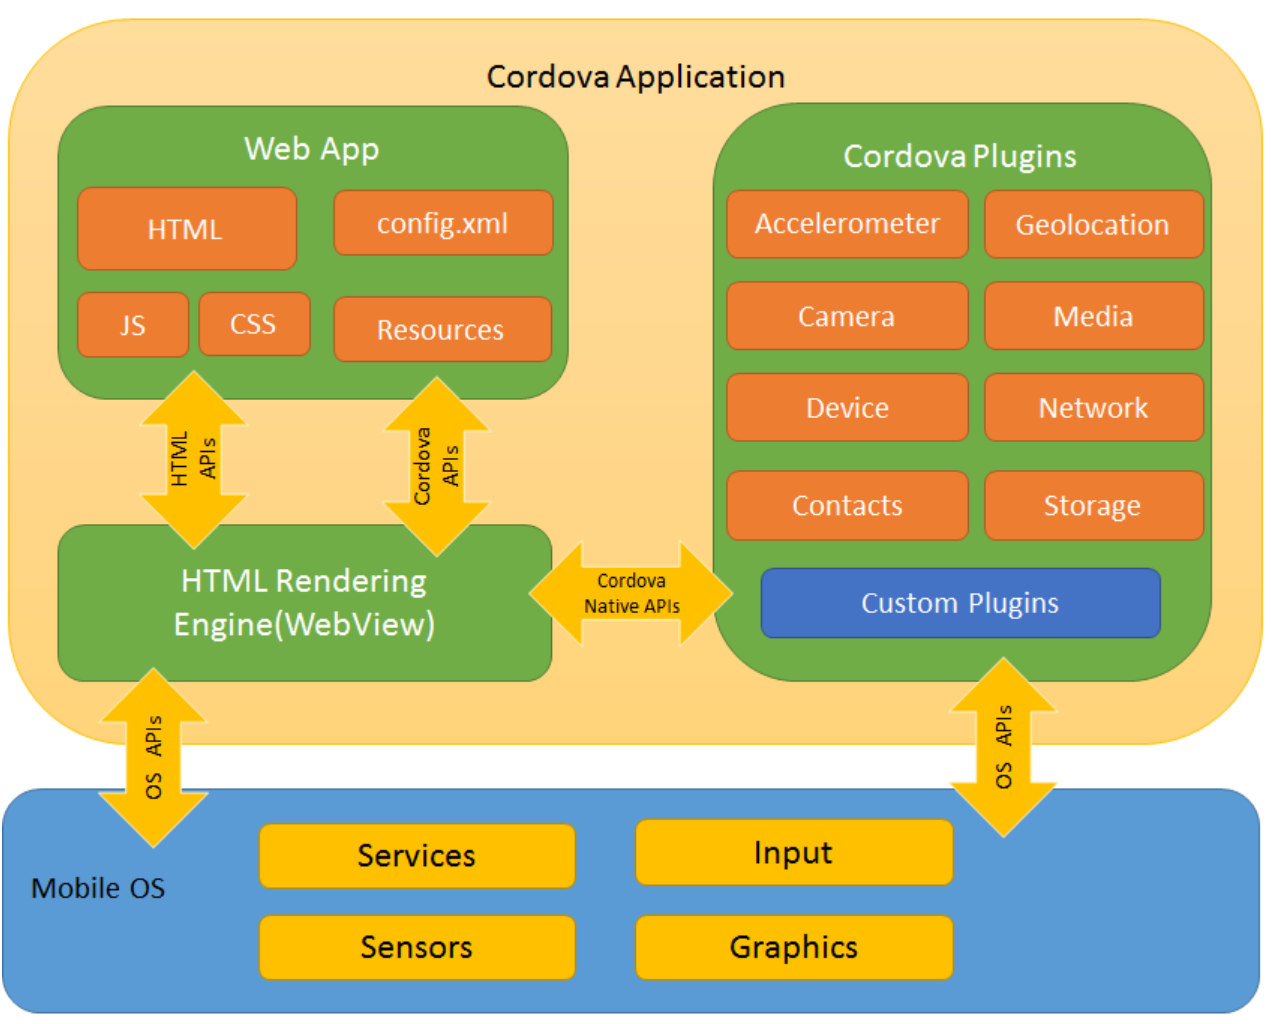
\includegraphics[width=0.75\textwidth]{cordova_architecture.png}
    \caption{Überblick über die Architektur einer Cordova-Anwendung \cite{Cordova_Overview}.}
    \label{fig:cordova_architecture}
\end{figure}
Die WebView ist ein eingebetteter Webbrowser, der vom Betriebssystem bereitgestellt wird \cite{Steyer_Cordova}.
Die Web-App kann Cordova-\acp{API} nutzen, um über die WebView auf Plugins zuzugreifen.
Diese Plugins bestehen aus einer JavaScript-Schnittstelle und einer plattformspezifischen nativen Implementierung.
Aufrufe der Funktionen eines Plugins werden in der WebView zu Aufrufen der nativen Implementierung aufgelöst \cite{Steyer_Cordova,Heitkoetter_CrossPlatform_Comparison}.
Für häufig verwendete Gerätefunktionen und \acp{API} stellt die Apache Software Foundation einige offizielle Plugins zur Verfügung.
Für eine Vielzahl von weiteren Funktionen sind Open-Source Plugins von anderen Anbietern verfügbar. 
Darüber hinaus erlaubt das Framework die Entwicklung eigener Plugins \cite{Cordova_Overview}.
Damit lassen sich alle Gerätefunktionen uneingeschränkt nutzen und bei Bedarf lässt sich die Performance von kritischer Funktionalität durch die Auslagerung in ein Plugin steigern.
Allerdings muss die Plugin-Funktionalität für jede zu unterstützende Zielplattform neu implementiert werden \cite{Steyer_Cordova}.

Werden Funktionen benötigt, für die keine Plugins verfügbar sind, steigt der Entwicklungsaufwand durch die Entwicklung eigener Plugins für jede zu unterstützende Plattform deutlich an.
Damit der große Vorteil der Cross-Plattform Entwicklung erhalten bleibt, sollten so wenige spezifische Plugins entwickelt werden müssen wie möglich.


Capacitor wurde 2018 von Ionic als modernere Alternative zu Cordova vorgestellt.
Wie Cordova, setzt Capacitor auf die Ausführung von Web-Apps in einer WebView innerhalb einer plattformspezifischen Wrapper-App.
Um den Umstieg von Cordova auf Capacitor zu erleichtern, können alle Cordova-Plugins direkt in Capacitor-Projekte eingebunden werden \cite{Liebel_Cordova_Capacitor}.
Für viele häufig verwendete Funktionen, stellt Ionic eigene Plugins für Capacitor zur Verfügung, deren Wartung und Support das Unternehmen übernimmt.
Zudem erlaubt Capacitor durch ein geändertes Build-Konzept eine einfachere Integration von nativem Code, ohne den Einsatz von Plugins \cite{Ionic_Cordova_vs_Capacitor}.
In Cordova-Projekten werden die nativen Projekte für die Wrapper-Anwendungen beim Build erzeugt und der Web-Code in diese eingebettet.
Bei Capacitor-Projekten werden die nativen Projekte für die Wrapper-Anwendungen bereits zu Beginn erstellt und sollen in die Versionsverwaltung aufgenommen werden.
Dadurch kann nativer Code direkt in die jeweiligen nativen Projekte integriert werden und wird nicht beim nächsten Build überschrieben \cite{Liebel_Cordova_Capacitor}.


Die Performance von Ionic und Cordova-basierten Anwendungen gilt allgemein als niedrig.
Bei reinen Cordova-Anwendungen wird zusätzlich die Konsistenz der \ac{UI} häufig kritisiert \cite{Steyer_Cordova}.
Beides ist auf die Einbettung von Web-Apps in native Wrapper-Anwendungen zurückzuführen.
Durch die Interpretation von JavaScript-Code innerhalb der WebView und den aufwändigen Zugriff auf native Funktionen über das komplexe Plugin-System, liegt die Performance von Cordova-Anwendungen deutlich unter der von nativen Anwendungen und häufig auch unter der von anderen Frameworks \cite{Rieger_CrossPlatform_EvaluationFramework,Biorn-Hansen_PerformanceOverhead_CrossPlatform}.


Capacitor ist trotz geringerer Verbreitung deutlich beliebter als Cordova \cite{Stackoverflow_2022,Appfigures_TopSDKs}.
Von allen Entwicklern, die bereits mit Capacitor gearbeitet haben, geben 62,35 \% an, das Framework auch weiterhin einsetzen zu wollen.
Nur 28,85 \% wollen Cordova weiter verwenden.
Damit schneidet Cordova von allen betrachteten Cross-Plattform Frameworks am schlechtesten ab.